\documentclass[12pt]{article}
\usepackage{fullpage,url,amssymb,epsfig,color,xspace,tikz,amsmath, amsthm}
\usepackage{graphicx}
\begin{document}

\begin{center}
    \textbf{\large Tutorial 1}
\end{center}

\section{student environment set up}
\begin{enumerate}
    \item First download Putty
    \begin{figure}[tbhp]
        \begin{center}
            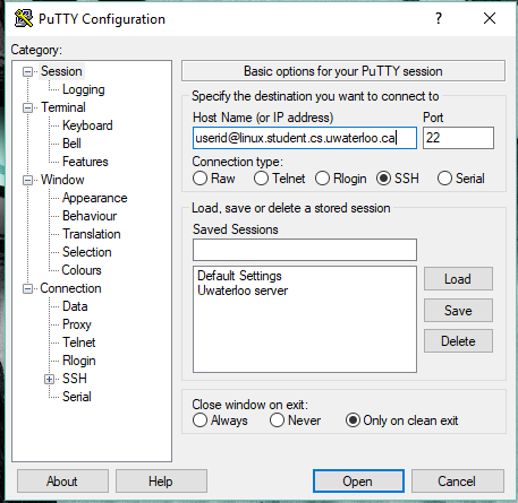
\includegraphics[width=0.5\textwidth]{Picture1.png}
        \end{center}
    \end{figure}

    \item Login with the information from your CS account
    \begin{figure}[tbhp]
        \begin{center}
            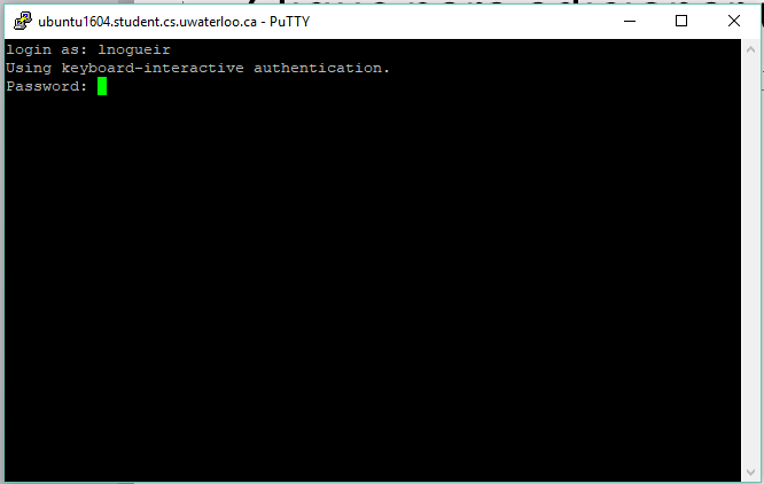
\includegraphics[width=0.5\textwidth]{Picture2.png}
        \end{center}
    \end{figure}
    \item create a new directory to store your files, strat editing your file using vim
    \begin{figure}[tbhp]
        \begin{center}
            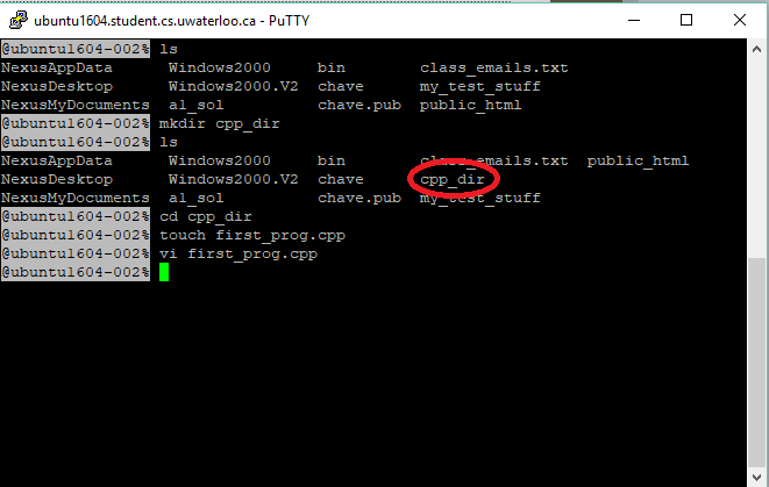
\includegraphics[width=0.5\textwidth]{Picture3.png}
        \end{center}
    \end{figure}
\end{enumerate}

\section{Compiling your programs}
command: g++ -std=c++14 -wall XXX.cc -o YYY\\
-std=c++14: compile using version c++14\\
-wall: dsiplay warning\\
-o: output file(defult as a.out)

\section{set of problems}
\begin{enumerate}
    \item What is the output of this function?
    \begin{verbatim}
#include <iostream>
#include <string>
#include <vector>
using namespace std;

int main() {
  string str;
  vector<string> v;
  while(!cin.eof()) {
    getline(cin, str);
    v.push_back(str);
    if(str == "") {
      cout << "empty" << endl;
    }
  }
  cout << v.size() << endl;
}
    \end{verbatim}

    \begin{enumerate}
        \item
        \begin{verbatim}
        Input: abcd\n\nEOF   
        Output:
        empty
        empty
        3
        \end{verbatim}
        \item
        \begin{verbatim}
        Input: abcd\nEOF   
        Output:
        empty
        2
        \end{verbatim}
    \end{enumerate}
    What about
    \begin{verbatim}
#include <iostream>
#include <string>
#include <vector>
using namespace std;
        
int main() {
  string str;
  vector<string> v;
  while(getline(cin, str)) {
    v.push_back(str);
    if(str == "") {
      cout << "empty" << endl;
    }
  }
  cout << v.size() << endl;
  }
    \end{verbatim}

    \begin{enumerate}
        \item
        \begin{verbatim}
        Input: abcd\n\nEOF   
        Output:
        empty
        2
        \end{verbatim}
        \item
        \begin{verbatim}
        Input: abcd\nEOF   
        Output:
        1
        \end{verbatim}
    \end{enumerate}

    \item Create a function that reads a text file and store the values of each line in a vector.
    \item Create a function that gets the entires of a vector and stores them in a text file.
    \item Create a function that given a text file with names, creates another text file with 
    the names sorted in alphabetical order.
\end{enumerate}

\begin{verbatim}
    #include <string>
    #include <vector>
    #include <fstream>
    #include <iostream>
    #include <algorithm>
    using namespace std;
    
    void storeVals(vector<string> &vals, string &file) {
      ifstream input;
      string str;
      input.open(file);
      if(!input.good()) {
        return;
      }
      while(input >> str) {
        vals.push_back(str);
      }
      input.close();
    }
    
    void OutputVals(vector<string> & vals, string &file) {
      ofstream output;
      if(file.find(".txt") == string::npos) {
        cerr << "File should be .txt" << endl;
        exit(1);
      }
      output.open(file);
      int size = vals.size();
      for(int i = 0; i < size; ++i) {
        output << vals[i] << endl;
      }
      output.close();
    }
    
    int findMin(vector<string> &vals, int begin) {
      int min = begin, size = vals.size();
      for(int i = begin + 1; i < size; ++i) {
        if(vals[min] > vals[i]) {
          min = i;
        }
      }
      return min;
    }
    
    void swap(vector<string> &vals, int i, int j) {
      string temp = vals[i];
      vals[i] = vals[j];
      vals[j] = temp;
    }
    
    void sortNames(vector<string> &vals) {
      //sort(vals.begin(), vals.end());
      int size = vals.size();
      for(int i = 0; i < size; ++i) {
        int min = findMin(vals, i);
        swap(vals, i, min);
      }
    }
    
    int main() {
      string nameIn ,nameOut;
      cin >> nameIn >> nameOut;
      vector<string> names;
      storeVals(names, nameIn);
      sortNames(names);
      OutputVals(names, nameOut);
      return 0;
    }
\end{verbatim}
\end{document}